%%%%%%%%%%%%%%%%%%%%%%% file template.tex %%%%%%%%%%%%%%%%%%%%%%%%%
%
% This is a template file for Web of Conferences Journal
%
% Copy it to a new file with a new name and use it as the basis
% for your article
%
%%%%%%%%%%%%%%%%%%%%%%%%%% EDP Science %%%%%%%%%%%%%%%%%%%%%%%%%%%%
%
%%%\documentclass[option]{webofc}
%%% "twocolumn" for typesetting an article in two columns format (default one column)
%
\documentclass{webofc}
\usepackage[varg]{txfonts}   % Web of Conferences font
%
% Put here some packages required or/and some personnal commands
%
%
\begin{document}
%
\title{A prototype for the evolution of Atlas Eventindex based on Apache Kudu storage}
%
% subtitle is optionnal
%
%%%\subtitle{Do you have a subtitle?\\ If so, write it here}

\author{\firstname{Zbigniew} \lastname{Baranowski}\inst{1}\fnsep\thanks{\email{zbigniew.baranowski@cern.ch}} \and
        \firstname{Luca} \lastname{Canali}\inst{1}\fnsep\thanks{\email{luca.canali@cern.ch}} \and
        \firstname{Alvaro} \lastname{Fernandez Casani}\inst{2}\fnsep\thanks{\email{Alvaro.Fernandez@ific.uv.es}} \and
        \firstname{Elizabeth} \lastname{Gallas}\inst{3}\fnsep\thanks{\email{elizabeth.gallas@physics.ox.ac.uk}} \and
        \firstname{Carlos} \lastname{Garcia Montoro}\inst{2}\fnsep\thanks{\email{carlos.garcia@ific.uv.es}} \and
        \firstname{Santiago} \lastname{González de la Hoz}\inst{2}\fnsep\thanks{\email{sgonzale@ific.uv.es}} \and
        \firstname{Julius} \lastname{Hrivnac}\inst{4}\fnsep\thanks{\email{Julius.Hrivnac@cern.ch}} \and
        \firstname{Fedor} \lastname{Prokoshin}\inst{5}\fnsep\thanks{\email{Fedor.Prokoshin@cern.ch}} \and
        \firstname{Grigori} \lastname{Rybkine}\inst{5}\fnsep\thanks{\email{Grigori.Rybkine@cern.ch}} \and
        \firstname{Jose} \lastname{Salt}\inst{5}\fnsep\thanks{\email{Jose.Salt@ific.uv.es}} \and
        \firstname{Javier} \lastname{Sanchez}\inst{5}\fnsep\thanks{\email{Javier.Sanchez@ific.uv.es}} \and
        \firstname{Dario} \lastname{Barberis}\inst{2}\fnsep\thanks{\email{Dario.Barberis@cern.ch}} 
        on behalf of the Atlas Collaboration
        % etc.
}




\institute{CERN, Geneva, Switzerland 
\and
           Insitut de Fisica Corpuscular, Valencia Spain 
\and
           University of Oxford, Oxford, UK
\and
           LAL, Université Paris-Sud and CNRS/IN2P3, Orsay, France
\and
           Universidad Tecnica Federico Santa Maria, Chile 6)Università di Genova and INFN, Genova, Italy
          }

\abstract{%
  The ATLAS EventIndex has been in operation since the beginning of LHC Run 2 in 2015. Like all software projects, its components have been constantly evolving and improving in performance. The main data store in Hadoop, based on MapFiles and HBase, can work for the rest of Run 2 but new solutions are explored for the future. Kudu offers an interesting environment, with a mixture of BigData and relational database features, which look promising at the design level and is used to build a prototype to measure the scaling capabilities as functions of data input rates, total data volumes and data query and retrieval rates. In this paper we report on the selected data schemas and on the current performance measurements with the Kudu prototype.
}
%
\maketitle
%
\section{Introduction}
\label{intro}
The ATLAS EventIndex is a catalogue of all real and simulated events produced by the experiment at all processing stages \cite{RefEI}. 
The system contains hundreds of billions of event records (180 billions of records as of June 2018), each consisting of approximately 1000 bytes. 
The goal of the ATLAS EventIndex is to allow fast and efficient selection of events of interest, based on various criteria, and provide references that point to those events in millions of files scattered in a world-wide distributed computing system.

\section{Motivation for the project evolution}
\label{sec-2}
Current EventIndex was designed in 2012-2013 using best BigData technology available at that time (Hadoop), implemented in 2014 using MapFiles and HBase, in operation since 2015 with satisfactory results \cite{RefEI2}.
However, the use cases evolved in the meantime and have been extended  from event picking and production completeness checks to trigger overlap studies, duplicate event detection and derivation streams (offline triggers) overlaps.
At the same time the implementation of fast data querying based on traditional relational database involves only a subset of information and is available for real events only \cite{RefORA}
Also event rate increased steadily throughout Run 2. \newline
BigData technologies advanced, in the meantime and now we have the choice between many different products and options.  
Studies of new data formats and/or new storage technologies \cite{RefZB} concluded that Kudu is the most promising technology for the next few years. Hence this prototype.

\section{Apache Kudu}
\label{sec-3}
Apache Kudu is a next generation scalable and distributed table-based storage designed for HTAP systems – Hybrid Transactional and Analytical Processing \cite{RefKudu}.
Unlike most of the data formats available for the Hadoop Distributed File System (HDFS), Kudu provides indexing and columnar data organization natively – this is to establish a good compromise between random data lookups and analytics performance.
Organization of the data in shared tables with named columns, types and a primary index makes Kudu very attractive for systems with relational data models that needs to scale-out.
Apache Kudu is supported by top open-source frameworks for parallel data processing and computation including Apache Spark, Apache Impala, Apache Hive, MapReduce and others.

\section{Concept of the new Atlas EventIndex platform}
\label{sec-4}
\begin{figure}[h]
\centering
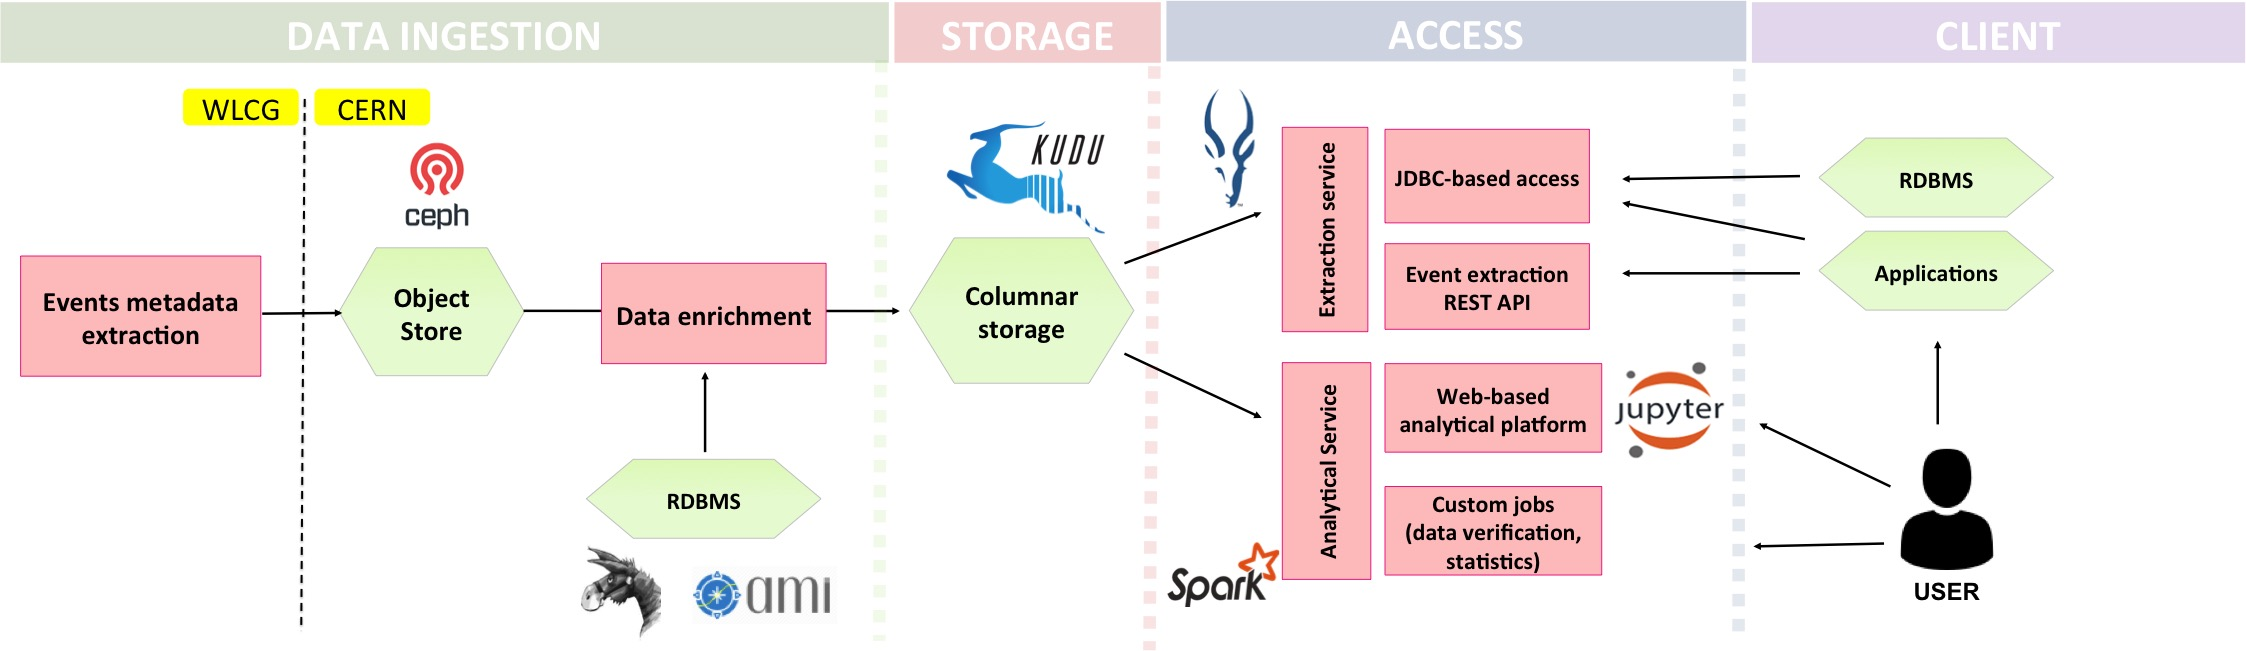
\includegraphics[width=\linewidth,clip]{architecture.jpg}
\caption{The new system architecture}
\label{fig:arch}
\end{figure}
Bringing on-board Kudu, a storage supported by many computing frameworks, offers to the project a possibility to have a modular architecture and increases its flexibility in further evolution. Any module responsible today for one of the the functions; data ingestion layer, data access layer or data analytic layer could be replaced with a modern one, without a significant effort. \newline
In the new architecture we foreseen to keep the data ingestion/production part without significant modification. It has been already modernized by introducing a staging area implemented with an object store layer \cite{CEPH} (based on Ceph storage) for all incoming indexed event data from WLCG \cite{WCG} jobs. The main work in this area is to build a data pipeline between the object store and the Kudu storage. Such pipeline will need to enrich the data with necessary information regarding trigger state, event provenance etc. from AMI \cite{AMI} and Rucio \cite{Rucio} systems. \newline
In order to fully profit from Kudu data access performance, the data access layer should be redesign. The MapReduce framework has to be replaced with low-latency SQL-based frameworks like Apache Impala. Impala is well integrated with Kudu and allow to start a lookup events queries within milliseconds. Moreover, the addition of SQL interface on to of Atlas Event Index data will open a possibility to integrate the project with external tools and systems over JDBC protocol. So eventually currently available web front-ends implemented for a relational back-end can be reconnected to the Kudu-based storage. \newline 
As more analytic use cases have been added to the system recently we would like implement them with Apache Spark, a modern, highly scale-able and feature-reach data processing engine. With Spark a lot of complex computations can be expressed in much easier way than with SQL. Finally, thanks to available integration of Spark with online Jupyter Notebooks (CERN's SWAN project \cite{SWAN}) we can empower the end-users to write their own analyses and executed on Atlas EventIndex data.
\section{Schema design in Apache Kudu}
\label{sec-5}
When designing a schema in Kudu one, has to make decision on the number of tables and relations between them, choosing appropriate primary keys and partitioning. The above have a crucial impact on the access time, scalability and usability of the data stored in Kudu. \newline
In this section we will describe the schema for Kudu tables that we prototyped to store the Atlas EventIndex data and the some criteria that led us to make certain design chooses.
\subsection{Technology constraints}
\label{sec-5-cons}
Along quite some limitations \cite{KuduLimitations} of Apache Kudu, there are few that impose certain schema design constraints. Notable, 1) each table has only one index and it is build on a primary key. 2) A table partition is a unit of a table scan parallelism. 3) Each Kudu cluster node can only host 5000 partitions. 4) Partition range has to be known during creation and cannot be modified. 5) Cardinality of key-hash-based sub-partitioning is static and cannot be changed per each partition individually. 6) A table cannot have more than 256 columns. 
\subsection{Partitioning strategy}
\label{sec-5-part}
Knowing the constraints mentioned in the previous sections we have to applied few techniques to go around them. \newline
This mainly applies to the non-primary key data access. Such access path requires a scan of all table columns that are part of a query predicate (filtering clause) or projection (selection clause). This quite expensive  (when comparing to the index-based access) process can be executed by multiple parallel processes on the Kudu cluster and effectively speed up the response time. The more partitions (including sub-partitions) the input table has the bigger parallelism can be achieved - this is due to the feature 2) mentioned in the previous section. For a single range partition we have decided to have 8 hash-based sub-partitions. This will give at least 8 parallel table scanners when running queries that cannot use index to read the data. \newline    
Furthermore, in order to reduce the work done by scanners, the number of rows to be visited by the scannig operation can be narrowed/pruned to those stored in certain partitions. This can happen if a partitioning key is present in a filter predicate of a query. In theory 'runnumber' column from Atlas EventIndex data is the best candidate for a table partition key, as it exists in all the queries and it has very low selectivity, hence only few partitions will be chosen for scanning. However, since the amount of data per run number is skewed we would have too many almost empty partitions and sub-partitions too. We could group more runs into single partition in order to keep all partitions with a unified size, however, due to the limitation 4) grouping cannot be done dynamically. To overcome the problem of statically defined partition keys we have introduce an artificial partition key for event data. Its value is an incremental number, and it has to be controlled by data ingestion supervisor. Once certain partition is big enough a new one should be created with a key incremented by one. Relation between partition keys and datasets has to be kept in a metadata table and looked up by each query. 
\subsection{Tables}
\label{sec-5-tables}
\begin{figure}
\centering
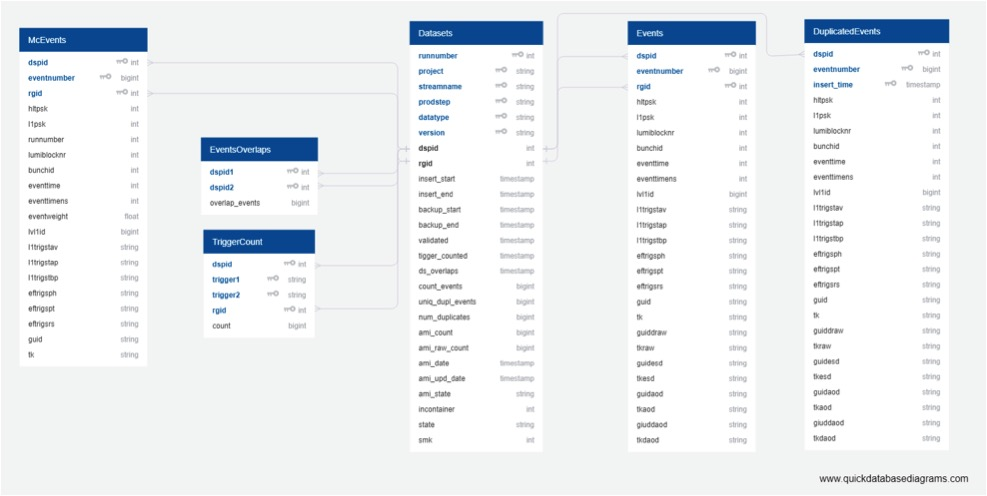
\includegraphics[width=\linewidth,clip]{schema.jpg}
\caption{Prototype schema}
\label{fig:schema}
\end{figure}
\section{Performance of the prototype}
\label{sec-6}


\subsection{Data ingestion}
\label{sec-6-di}
\begin{figure}
\centering
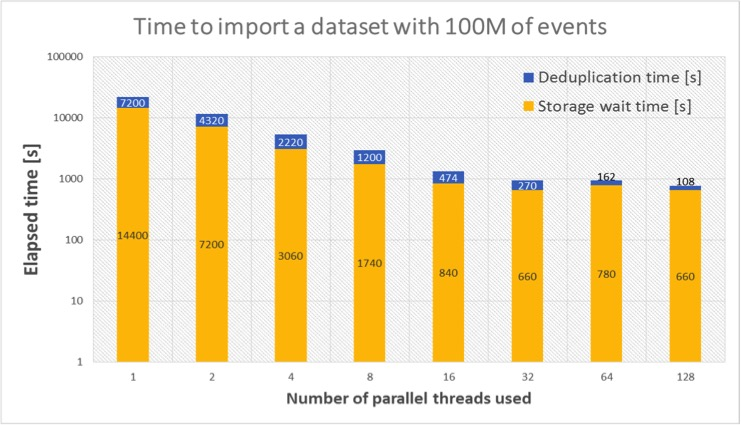
\includegraphics[width=\linewidth,clip]{ingestion.jpg}
\caption{Data ingestion speed measured on representative data set}
\label{fig:ingestion}
\end{figure}
Data loading tests were performed with Apache Spark 2.2.1 using real data from the current production system.
Before loading a dataset to Apache Kudu, duplicated events are filtered out and stored in a dedicated table. The performance test have been concluded on multiple datasets with random size and various number of parallel ingestion processes. 
Figure ~\ref{fig:ingestion} shows the results of the set of test performed on an representative dataset with 100M events to demonstrate scalability of data ingestion 
Measured average writing speed was 5kHz per thread, max overall writing speed to a Kudu cluster was 120kHz. The obtained result is ~10x more than what is needed today by the project.

\subsection{Data access}
\label{sec-6-da}
\begin{figure}
\centering
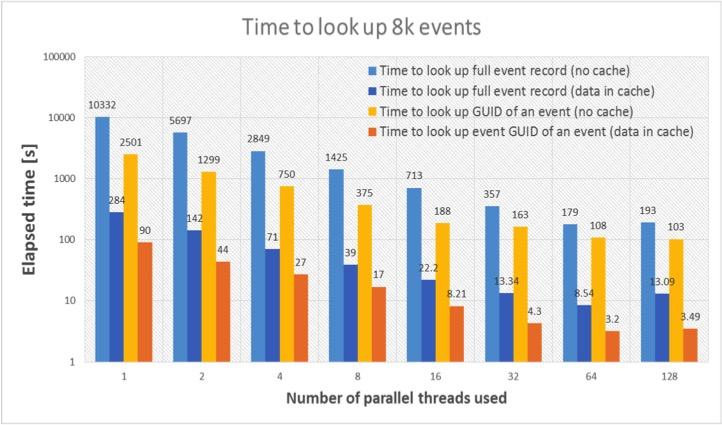
\includegraphics[width=\linewidth,clip]{data_access.jpg}
\caption{Data access representative data set}
\label{fig:access}
\end{figure}
On the Figure~\ref{fig:access} we present the time to look up eight thousands of random events records (full record or just a GUID attribute) from Apache Kudu with a simple client written in Python.
The results for each type of a lookup were grouped into two cases; a pessimistic one (no cache used ) and an optimistic one (all data where lookup from Kudu cache).
The average event lookup time below 1s and ability to handle more then 400 requests per second fully satisfies the future system needs. 

\subsection{Analytic}
\label{sec-6-an}
\begin{figure}
\centering
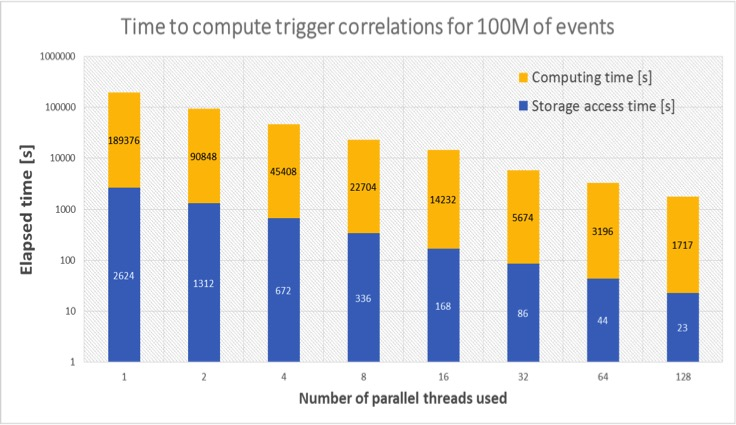
\includegraphics[width=\linewidth,clip]{analytics.jpg}
\caption{Data analytic speed measured on representative data set}
\label{fig:analytics}
\end{figure}
Data analytics tests were performed with Apache Spark 2.2.1 reading Atlas EventIndex from data stored in Apache Kudu.
In Figure~\ref{fig:analytics} are presented execution times for the test case, were we count the occurrences of all combinations of trigger bits pairs within a dataset of 100M events
The trigger count computation on a Spark cluster takes the majority of the wall time (52 hours), when data retrieval from Kudu is just a small fraction (< 2\%) of it (45 minutes). A single scanner thread could deliver 40k of records per second


\section{Summary}
\label{sec-7}
Scalable data scan performance in combination with modern data processors (Spark, Impala) opens the system to new use cases on a filed of data exploration and analytics (like counting trigger correlations)



\begin{thebibliography}{}

\bibitem{RefEI}
Barberis D et al. 2014 The ATLAS EventIndex: an event catalogue for experiments collecting 
\bibitem{RefEI2}
Barberis D et al. 2015 The ATLAS EventIndex: architecture, design choices, deployment and first operation experience, J. Phys. Conf. Ser. 664 042003
\bibitem{RefORA}
Gallas E et al. 2016 an Oracle-based Event Index for ATLAS

\bibitem{RefZB}
Z. Baranowski et al 2017 J. Phys.: Conf. Ser. 898 062020

\bibitem{RefKudu}
Lipcon T et al., 2015 Kudu: Storage for fast analytics on fast data.





% Format for Journal Reference
Journal Author, Journal \textbf{Volume}, page numbers (year)
% Format for books
\bibitem{RefB}
Book Author, \textit{Book title} (Publisher, place, year) page numbers
% etc
\end{thebibliography}

\end{document}

% end of file template.tex

<div id='footer'><table width='100%'><tr><td class='right'><a href='http://fusioninventory.org/'><span class='copyright'>FusionInventory 9.1+1.0 | copyleft <img src='/glpi/plugins/fusioninventory/pics/copyleft.png'/>  2010-2016 by FusionInventory Team</span></a></td></tr></table></div>